% !TEX Root = ../proposal.tex

\appendix
\section[Appendix]{Appendix}
\subsection[Gravity Models]{Gravitational Modelling}

\begin{frame}[noframenumbering,label=astro] %----------------------------------------------%
\frametitle{Astrodynamics}

\only<1>{
\begin{block}{Newton's Law of Universal Gravitation}
    Any two bodies attract one another with a force proportional to the product of their masses and invesely proportional to the square of the distance between them
    \[
    \vecbf{F} = - \frac{G m_1 m_2}{ r^2} \frac{\vecbf{r}}{r}
    \]
\end{block}
}
\only<2>{
\begin{block}{N-Body}
    Gravitational attraction of \( n \) bodies acting on the particle of interest \( m_i \)
    \[
    m_i \ddot{\vecbf{r}}_i = -G \sum_{\substack{j = 1\\j\neq i}}^n \frac{m_i m_j}{r_{ji}^3} \vecbf{r}_{ji}
    \]
    Motion of \( \bar{r}_j (t) \) is not known - Not solvable in general
    
\end{block}
}
\hyperlink{slide:system_model_challenges}{\beamergotobutton{Dynamic Challenges}}
\end{frame} %--------------------------------------------------------------%

\begin{frame}[noframenumbering,label=centrobaric]
\frametitle{Gravitational Modeling}
\begin{block}{Centrobaric Body}
    \( \vecbf{F} = -\frac{G m_1 m_2}{R^2} \vecbf{a}_1 \) for all particles outside of body
\end{block}

\begin{columns}
    \begin{column}{0.5\textwidth}
        \begin{itemize}
            \item<2-> Only applies to spherically symmetric bodies 
            \item<3-> \Emph{Gravity Model} requires accurate tracking of SC
                \begin{itemize}
                    \item Spherical Harmonic
                    \item Mass concentration
                    \item Polyhedron Potential
                \end{itemize}
        \end{itemize}
    \end{column}
    \begin{column}{0.5\textwidth}
        \visible<2->{
        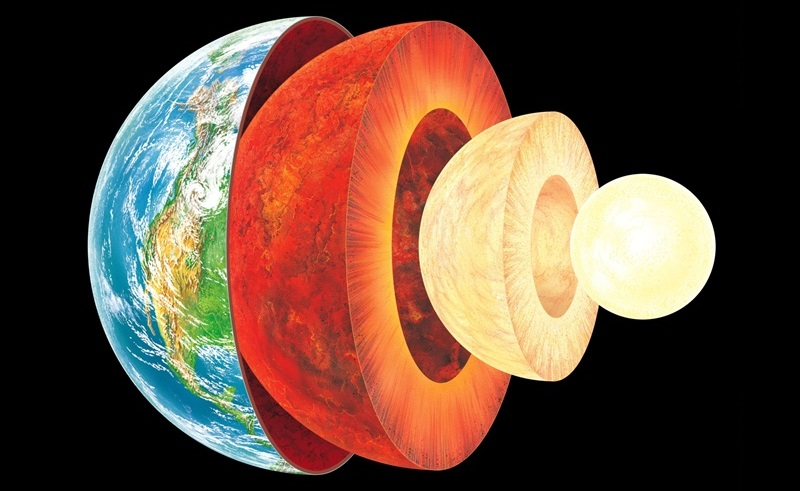
\includegraphics[width=\textwidth,height=0.5\textheight,keepaspectratio]{figures/earth_layers.jpg}
        }
    \end{column}
\end{columns}

\note[itemize]{
    \item Models require detailed data from orbit about asteroid (OD process determines gravity field)
    \item Simplified models (triaxial ellipsoid allows analytical insight)
    \item Previous work fails to consider coupled dyanmics
    }
\end{frame}

\begin{frame}[noframenumbering]{Polyhedron Gravitation Model}
\label{slide:polyhedron_gravity}
\begin{itemize}
    \item Potential is a function of only the shape model
    \item Globally valid, closed-form expression of potential
    \item Exact potential assumes a constant density 
    \item Accuracy solely dependent on shape model
\end{itemize}
\only<2>{
\begin{align*}\label{eq:potential}
    U(\vecbf{r}) &= \frac{1}{2} G \sigma \sum_{e \in \text{edges}} \vecbf{r}_e \cdot \vecbf{E}_e \cdot \vecbf{r}_e \cdot L_e - \frac{1}{2}G \sigma \sum_{f \in \text{faces}} \vecbf{r}_f \cdot \vecbf{F}_f \cdot \vecbf{r}_f \cdot \omega_f 
\end{align*}
}
\only<3>{
\begin{center}
  \animategraphics[controls,autoplay,loop,width=0.5\textwidth]{30}{animation/2016AAS/castalia/IMG}{00001}{00999}~\hfill
  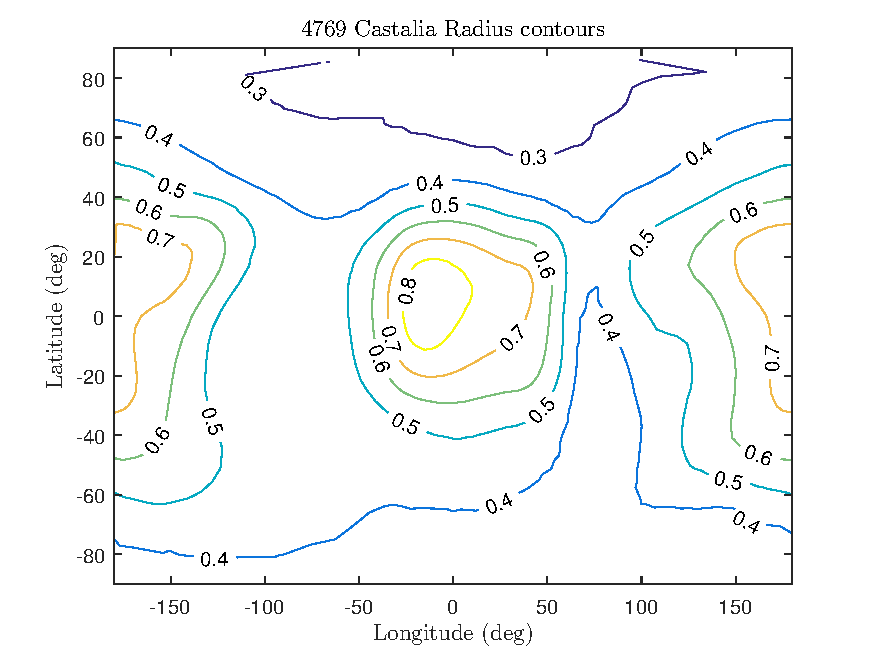
\includegraphics[width=0.5\textwidth]{figures/2016AAS/radius_contour.pdf}
\end{center}
}

\end{frame}

\begin{frame}[noframenumbering]{Astrodynamics}%-------------------------------------------------------%
\label{slide:astrodynamics}

\only<1>{
\begin{block}{Integrals of Motion}
    Require \( 6 n \) integrals of motion but know \( 10 \)
        \begin{itemize}
            \item Linear Momentum - system CM constant speed - \( 6 \) constants
            \item Angular Momentum - system angular moment - \( 3 \) constants
            \item Total Energy - Conservative system - \( 1 \) constant
        \end{itemize}
    Even two-body problem is not solvable
\end{block}
}
\only<2>{
\begin{block}{Relative Motion}
Really care about relative motion of \( m_i \) wrt \( m_q \)
\[
    \ddot{\vecbf{r}}_{qi} + G \frac{m_i + m_q}{r_{qi}^3} \vecbf{r}_{qi} = G \sum_{\substack{j = 1\\j\neq i,q}}^n m_j \parenth{ \frac{\vecbf{r}_{ij}}{r_{ij}^3} - \frac{\vecbf{r}_{qj}}{r_{qj}^3}} \vecbf{r}_{ji}
\]
\end{block}
}

\end{frame} %----------------------------------------------------------% 

\subsection{Attitude Coupling}

\begin{frame}[noframenumbering,label=grav] %---------------------------------------%
\frametitle{Gravity Expansion}
\only<1>{
\begin{block}{Force due to gravity on body \( B\) from particle \( P \)}
\begin{equation*}
    \vecbf{F} = -G m_P \int_{\mathcal{B}} \vecbf{r} \parenth{r^2}^{-\frac{3}{2}} \, d m
\end{equation*}
\end{block}
}
\only<2>{
\begin{block}{Binomial Expansion}

\begin{align*}
    \vecbf{F} &= - \frac{G m_P m_B}{R^2} \parenth{\vecbf{a}_1 + \sum_{i=2}^\infty \vecbf{f}^{(i)}} \\
    \vecbf{f}^{(2)} &= \frac{1}{m_B R^2} \braces{\frac{3}{2} \bracket{ \tr{J_B} - 5 \vecbf{a}_1 \cdot J_B \cdot \vecbf{a}_1} \vecbf{a}_1 + 3 J_B \cdot \vecbf{a}_1}
\end{align*}
\end{block}
}
\only<3>{
\begin{block}{Gravity Moment}
\begin{equation*}
    \vecbf{M} = \frac{3 G m_B}{R^3} \vecbf{a}_1 \times J \cdot \vecbf{a}_1 + \frac{G m_B m_P}{R} \sum_{i=3}^\infty \vecbf{a}_1 \times \vecbf{f}^{(i)}
\end{equation*}
%\begin{center}
%CG \( \neq \) CM 
%\end{center}
\end{block}
}

\end{frame}%-------------------------------------------------------------%


\begin{frame}[noframenumbering,label=srp]{Solar Radiation Pressure} %---------------------------------------------------%

\begin{block}{Constant Area Approximation}
Momentum transfer from solar photons striking spacecraft
\begin{align*}
    \vecbf{a}_{SRP} = - \frac{\parenth{1 + \rho} P_0 A_{S}}{M_S} \frac{\vecbf{d} - \vecbf{r}}{\norm{\vecbf{d}-\vecbf{r}}^3}
\end{align*}

\( P_0\) is a solar flux constant \SI{1e8}{\kilogram\kilo\meter\cubed\per\second\squared\per\meter\squared}

\( B_S = \frac{M_S}{A_S} \) is a mass to area ratio - \( 20 - 40 \, \si{\kilogram\per\meter\squared} \)

\( \rho \) is total reflectance or albedo of body

\( \vecbf{d}, \vecbf{r} \) defined in small body frame to Sun and S/C respectively
\end{block}
\begin{itemize}
    \item Large bodies, i.e. 433 Eros, SRP may be neglected
    \item Small bodies, \( < 1-5 \si{\kilo\meter} \), SRP is crucial
\end{itemize}
\end{frame} %-----------------------------------------------------------%

\subsection{Dynamics}

\begin{frame}[noframenumbering]{Lagrange's Equations}%---------------------------------------------%
\label{slide:lagrange}
\begin{block}{Conservative System}
  All applied forces \( \vecbf{F}_i \) are derivable from a potential function \( V(x_1, x_2, \ldots, x_{3N}) \) : \(\vecbf{F}_i = -\deriv{V}{\vecbf{x}_i}\)
\end{block}

\only<1>{
\begin{block}{Hamilton's Principle}
    The actual path in configuration space followed by a holonomic system during the fixed interval \( t_0 \) to \( t_1\) is such that the action integral:
    \[
    S = \int_{t_0}^{t_1} L(q, \dot{q}) dt
    \]
    is stationary with respect to path variations which vanish at the end-points.
\end{block}
}
\only<2>{
\begin{block}{Variation of action integral}
\begin{align*}
    \delta S &= \int_{t_0}^{t_1} \deriv{L}{q} \delta q + \deriv{L}{\dot{q}} \delta \dot{q} \, dt \\
        &= \int_{t_0}^{t_1} \deriv{L}{q} \delta q - \frac{d}{dt} \left( \deriv{L}{\dot{q}}\right) \delta q \, dt - \left. \left[ \deriv{L}{\dot{q}} \delta q\right] \right|_0^T \\
    &= \int_{t_0}^{t_1} \deriv{L}{q} - \frac{d}{dt} \left( \deriv{L}{\dot{q}}   \right) \, dt \, ,
\end{align*}
\end{block}
}
\end{frame}%---------------------------------------------------------------------------%

\begin{frame}[noframenumbering]{Jacobi Integral}
\label{slide:jacobi}
\only<1>{
\begin{block}{Total Mechanical Energy}
\begin{enumerate}
    \item Generalized force from potential function: \( Q_i = -\deriv{V}{q_i} \)
    \item Work is path independent: \( W = \sum_{i=1}^{n} \int_{A_i}^{B_i} Q_i \, dq_i \)
\end{enumerate}

    If no other forces do work, then total mechanical energy is conserved:  \(  E(q, \dot{q}) = T + V   \)
\end{block}
}
\only<2>{
\begin{block}{More general constant}
\begin{enumerate}
    \item Standard Form of Lagrange's equation applies
    \item Lagrangian is not explicit fcn of time
    \item Constraints may be expressed: \( \sum_{i=1}^n a_{ji} d q_i = 0\)
\end{enumerate}

\[
    h = \sum_{i=1}^n \deriv{L}{\dot{q}_i} \dot{q}_i - L 
\]
\end{block}
}

\end{frame} %-----------------------------------------------------------%

\begin{frame}[noframenumbering] %------------------------------------%
\frametitle{Variational Principle}
    \begin{itemize}
        \item Variational Integrators
            \begin{itemize}
                \item Structure-preserving integrators for Hamiltonian systems
                \item Obtained by discretizing variational principle
            \end{itemize}
    \end{itemize}
    \pause
    \begin{columns}[c]
        \begin{column}{0.5\textwidth}
            \centering
            \begin{beamercolorbox}[wd=0.8\columnwidth,sep=0.05cm,center]{numerical} Continuous Time \end{beamercolorbox}
            \begin{beamercolorbox}[wd=0.8\columnwidth,sep=0.05cm,center]{numerical} 
                Configuration Space \\
                \( \parenth{q, \dot{q} } \in TQ \)
            \end{beamercolorbox}
            \begin{beamercolorbox}[wd=0.8\columnwidth,sep=0.05cm,center]{numerical} 
                Lagrangian \\
                \( L\parenth{q, \dot{q} } \)
            \end{beamercolorbox}
            \begin{beamercolorbox}[wd=0.8\columnwidth,sep=0.05cm,center]{numerical} 
                Action Integral \\
                \( S = \int_{0}^T L\left( q, \dot{q}\right) \, dt \)
            \end{beamercolorbox}
            \begin{beamercolorbox}[wd=0.8\columnwidth,sep=0.05cm,center]{numerical} 
                Stationary Action \\
                \( \delta S = 0 \)
            \end{beamercolorbox}
%           \begin{beamercolorbox}[wd=0.8\columnwidth,sep=0.05cm,center]{numerical} 
%               Legendre Transform \\
%               \( p_i = \deriv{L}{\dot{q}} \)
%           \end{beamercolorbox}
            \begin{beamercolorbox}[wd=0.8\columnwidth,sep=0.05cm,center]{numerical} 
                Equation of Motion \\
                \( \ddot{q} = f \parenth{q, \dot{q} } \)
            \end{beamercolorbox}
        \end{column}
        \pause
        \begin{column}{0.5\textwidth}
            \centering
            \begin{beamercolorbox}[wd=0.8\columnwidth,sep=0.05cm,center]{numerical} Discrete Time \end{beamercolorbox}
            \begin{beamercolorbox}[wd=0.8\columnwidth,sep=0.05cm,center]{numerical} 
                Configuration Space \\
                \( \parenth{q_k, q_{k+1} } \in Q \times Q \)
            \end{beamercolorbox}
            \begin{beamercolorbox}[wd=0.8\columnwidth,sep=0.05cm,center]{numerical} 
                Lagrangian \\
                \( L_d\parenth{q_k, q_{k+1}} \)
            \end{beamercolorbox}
            \begin{beamercolorbox}[wd=0.8\columnwidth,sep=0.05cm,center]{numerical} 
                Action Sum \\
                \( S_d = \sum_{k=0}^{N-1} L_d(q_k, q_{k+1}) \)
            \end{beamercolorbox}
            \begin{beamercolorbox}[wd=0.8\columnwidth,sep=0.05cm,center]{numerical} 
                Stationary Action \\
                \( \delta S_d = 0 \)
            \end{beamercolorbox}
%           \begin{beamercolorbox}[wd=0.8\columnwidth,sep=0.05cm,center]{numerical} 
%               Fiber Derivative \\
%               \( p_k = - \deriv{L_d(q_k, q_{k+1})}{q_k} \) \\
%               \( p_{k+1} = \deriv{L_d(q_k, q_{k+1})}{q_{k+1}} \)
%           \end{beamercolorbox}
            \begin{beamercolorbox}[wd=0.8\columnwidth,sep=0.05cm,center]{numerical} 
                Equation of Motion \\
                \( q_{k+2} = f_d \parenth{q_k, q_{k+1} } \)
            \end{beamercolorbox}
        \end{column}
    \end{columns}
    
    \note[itemize]{
        \item Continous time - discretization occurs at end while implemented in digital computer
        \item Discrete time - discretization occurs at the beginning. 
        Dynamics derived in discrete time
        \item Legendre transform allows for expression of dynamics in Hamiltonian form
    }
\end{frame}%-----------------------------------------%

\begin{frame}[t,noframenumbering]{Dynamics of Rigid Body} %------------------------------------------------%
    \begin{block}{Newton's Law}
        
        \begin{align*}
            F_x &= m \parenth{\dot{v}_x + v_z \omega_y - v_y \omega_z} \\
            F_y &= m \parenth{\dot{v}_y + v_x \omega_z - v_z \omega_x} \\
            F_z &= m \parenth{\dot{v}_z + v_y \omega_x - v_x \omega_y} \\
        \end{align*}
    \end{block}
    
    \begin{block}{Euler's Law}
        \begin{align*}
            {M}_x &= I_{xx} \dot{\omega}_x + \parenth{I_{zz}-I_{yy}} \omega_y \omega_z \\
            {M}_y &= I_{yy} \dot{\omega}_y + \parenth{I_{xx}-I_{zz}} \omega_z \omega_x \\
            {M}_z &= I_{zz} \dot{\omega}_z + \parenth{I_{yy}-I_{xx}} \omega_x \omega_y \\
        \end{align*}
    \end{block}
\end{frame} %----------------------------------------------------------------------%

\begin{frame}[noframenumbering]{Spacecraft Propulsion}\label{slide:propulsion}%------------------------------------------------%
\begin{block}{Ideal Rocket Equation}
    Amount of propellant required for a given velocity change
    \[
        \Delta V = - g_0 I_{sp} \ln\parenth{\frac{m_f}{m_i}}
    \]
\end{block}

\begin{itemize}
    \item High exhaust speeds make electric propulsion attractive
    \item Much higher efficiency than chemical propulsion
\end{itemize}
\hyperlink{slide:lowthrust_vehicles}{\beamergotobutton{Low-Thrust Vehicles}}

\end{frame} %----------------------------------------------------------------%

% Differences when considering an asteroid - polyhedron model

\subsection{Attitude Kinematics}
\begin{frame}[noframenumbering]{Attitude Kinematics}
\label{slide:attitude_kinematics}

\begin{columns}
\begin{column}{0.5\textwidth}
\begin{itemize}
    \item Many ways to represent the orientation of a rigid body
    \begin{itemize}
        \item Conceptual simplicity
        \item Computational considerations
        \item Legacy hardware/code
        \item Mathmatical simplicity/convience
    \end{itemize}
\end{itemize}
\end{column}
\pause
\begin{column}{0.5\textwidth}
    \begin{itemize}
        \item Euler axis and angle (4)
        \item Rotation Matrix (9)
        \item Euler angles (3)
        \item Quaternion (4)
        \item Rodriguez Parameters (4)
        \item Modified Rodriguez parameters (4)
    \end{itemize}
\end{column}
\end{columns}
\pause
\begin{block}{Minimal Representations}
    All minimal attitude representations have kinematic singularities and are not suitable for large rotations.
\end{block}

\hyperlink{slide:attitude_control}{\beamergotobutton{Attitude Control}}
\end{frame}

\begin{frame}[noframenumbering]{Attitude Parameterizations}
\label{slide:attitude_parameterizations}
    \begin{itemize}
        \item Euler Angles
        \begin{itemize}
            \item Minimal representation used for small attitude changes.
            \item Singularities exist for large angle slews: requires switching between 24 sequences
            \item Complicated trigonometric functions
        \end{itemize}
        \pause
        \vs
        \item Quaternion 
        \begin{itemize}
            \item No singularities
            \item Two anti-podal quaternions for the same attitude
            \item Unwinding behavior for control systems
        \end{itemize}
        \pause
        \vs
        \item Geometric control
        \begin{itemize}
            \item Globally and uniquely characterize attitude: \( R \in \SO \)
            \item Controller is globally valid for large angle maneuvers
        \end{itemize}
    \end{itemize}

\end{frame}

\begin{frame}[t,noframenumbering]\frametitle{Constrained Attitude Control}
\label{slide:attitude_constraints}
    \begin{itemize}
    \item \Emph{Constrained attitude control} : reorient vehicle while avoiding pointing at obstacles
    \begin{itemize}
        \item Exclusion zones for payloads e.g infrared telescope
        \item UAVs manuevering in congested locations
        \item Laser/Radio emitters on spacecraft
    \end{itemize}
    \pause
    \vs
    \item Previous approaches have several issues
    \begin{itemize}
        \item Attitude parameterizations: singularities/ambiguities
        \item Ad-hoc path planning: difficult to generalize to arbitrary obstacles
        \item Randomized methods: lack of stability guarantees
        \item Optimization based: expensive to compute and only provides open-loop control  
    \end{itemize}
\end{itemize}


\end{frame}